\documentclass[a4paper]{report}
\usepackage[utf8]{inputenc}
\usepackage[T1]{fontenc}
\usepackage{RJournal}
\usepackage{amsmath,amssymb,array}
\usepackage{booktabs}
\usepackage{float}
\usepackage{Sweave}
\usepackage[parfill]{parskip}

%\VignetteEngine{Sweave}
%\VignetteIndexEntry{walkr}

\begin{document}

%% do not edit, for illustration only
\sectionhead{Contributed research article}
\volume{XX}
\volnumber{YY}
\year{20ZZ}
\month{AAAA}

\begin{article}

\title{walkr}

\author{by David Kane, Andy Yao}

\maketitle      

\abstract{
The \texttt{walkr} package samples points using random walks from the intersection of 
the $N$ simplex with $M$ hyperplanes. Mathematically, the sampling space is all vectors $x$ 
that satisfy $Ax=b$, $\sum x = 1$, and $x_i \geq 0$. The sampling algorithms implemented 
are hit-and-run and Dikin walk, both of which are MCMC (Monte-Carlo Markov Chain) random 
walks. \texttt{walkr} also provide tools to examine and visualize the convergence
properties of the random walks.

}

\section{Introduction} 

$A$ and $b$ represent the system of equations that we have above. Specifically, $A$ is a $M \times N$ matrix ($M$ variables and $N$ constraints), and $b$ is a $M \times 1$ vector.

\section{Mathematical Background of Sampling Space}

In this section, we go through the mathematical background needed to understand the space from which 
we are sampling -- the intersection of the $N$ simplex and 
hyperplanes. Specifically, we go through a few examples as well as some linear algebra 
tricks. The reader does not need to read this section in order to use our package or understand
our sampling algorithms. However, this section should help the reader understand better what 
the sample space is both geometrically and mathematically. \\

\noindent \textbf{Definition:} The $N$-dimensional unit simplex is described by:

$$x_1 + x_2 + x_3 + ... + x_n = 1$$
$$x_i \geq 0$$

\subsection{Sampling space: simple 3D case}

Let's begin with the simplest case -- one linear constraint in 3 dimensional space.

$$x_1 + x_3 = 0.5$$

We can express this in terms of matrix equation $Ax=b$, where:

$$
A = 
\begin{bmatrix}
1 & 0 & 1 \\
\end{bmatrix},
\quad
b = 0.5,
\quad
x = 
\begin{bmatrix}
x_1 \\
x_2 \\
x_3 \\
\end{bmatrix}
$$ 

In addition, we require the solution space to be intersected with the $3$D simplex: 

$$\sum x_i = 1$$
$$x_i \geq 0$$

In the following graph, we draw the intersection of the two. The orange equilateral triangle represents the 3D simplex, and the blue rectangle represents the plane $w_1+w_3=0.5$. The intersection of the hyperplane (blue) with the simplex (orange) is the red line segment, which is our sampling space.

% should probably replace this figure with a better one

\begin{figure}[H]
\centering
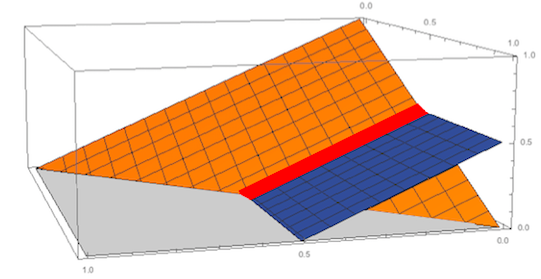
\includegraphics[width = 4in, height = 2.5in]{img/3Dcase.png}
\caption[caption]{Intersection (red line) of Simplex and 2D hyperplane living in 3D space}
\end{figure}

\subsection{Matrix Representation of Hyperplanes}

Every hyperplane is described by one linear equation. Thus, a system of linear equations is the intersection
of hyperplanes. In general, if we have $M$ linear equations and $N$ variables, then $Ax=b$ would look like:

$$
A_{M \times N} = 
\underbrace{
  \begin{bmatrix}
   & & & & & & \\
   & & & ... & & & \\
   & & & & & & \\
%    &  & . & . & . &  & \\
%    &  & . & . & . &  & \\
%    &  & . & . & . &  & \\
%    & & & & & & \\
  \end{bmatrix}
}_\text{N columns (variables)}
\Bigg\}\text{{M rows (constraints)}}
$$

$$
b = b_{M \times 1}, 
\quad
x = x_{N \times 1}
$$

\subsection{Going from $Ax=b$ and the unit-simplex to $Ax \leq b$}

Our sampling space is represented by equalities $Ax = b$, $\sum x = 1$, and non-negativity constraint
$x_i \geq 0$. Because of the inequality, our sampling space is bounded (i.e. has finite volume in 
$\mathbb{R}^N$). More formally, our sampling space known as a \textbf{convex-polytope} 
in $\mathbb{R}^N$, which
could be described by a generic $Ax \leq b$. Here, we describe a transformation which takes us 
from the intersection of $Ax=b$ and the unit-simplex to a large matrix inequality of the form
$Ax \leq b$. \\

First, note that the equality part of the simplex constraint could be added as an extra row 
in $Ax = b$

$$
A =
  \begin{bmatrix}
   & & ...... & & & \\
   & & ......  & & & \\
   & & ...... & & & \\
   & & & & & \\
   1 & 1 & ...... & 1 & 1 \\

  \end{bmatrix}, 
\quad 
b = 
  \begin{bmatrix}
    \\
   \\
  ... \\
   \\
  1 \\
  \end{bmatrix}
$$

Second, to find the complete solution to the new $Ax = b$ (i.e. the set of all possible $x$'s that satisfy
$Ax=b$), we must find the Null Space Basis of $A$, the set of all possible $x$'s that satisfy $Ax=0$, 
then add on a particular solution to $Ax = b$. \\

Mathematically, if the original $A$ was $M \times N$, then after adding on the extra row from the simplex, 
the set of basis vectors which span the Null Space of our new $A$ will be: 

$$v_1, \quad v_2, \quad v_3, \quad ...... \quad , \quad v_{M-(N+1)}$$

\noindent Third, using any particular solution, $v_{particular}$, the complete solution to the new $Ax=b$
will be 

$$
\Bigg\{
v_{particular} + \alpha_1v_1 + \alpha_2v_2 + \alpha_3v_3 + ... + \alpha_{M-(N+1)}v_{M-(N+1)}
\quad | \quad \alpha_i \in \mathbb{R}
\Bigg\}
$$ \\ 

Lastly, we tag on the $x_i \geq 0$ constraints, and with some algebraic manipulations:

$$v_{particular} + \alpha_1v_1 + \alpha_2v_2 + \alpha_3v_3 + ... + \alpha_{M-(N+1)}v_{M-(N+1)}
\quad \geq
\begin{bmatrix}
0 \\
0 \\
... \\
... \\
... \\
0 \\
\end{bmatrix}
$$

$$
\alpha_1v_1 + \alpha_2v_2 + \alpha_3v_3 + ... + \alpha_{M-(N+1)}v_{M-(N+1)}
\quad \geq -v_{particular}
$$

$$
V\alpha \geq -v_{particular}, \quad \text{where:} \quad
V = 
\begin{bmatrix}
v_1 &
v_2 &
... &
v_{M-(N+1)} \\
\end{bmatrix}, 
\quad
\alpha = 
\begin{bmatrix}
\alpha_1 \\
\alpha_2 \\
... \\
\alpha_{M-(N+1)}
\end{bmatrix}
$$

\noindent And finally, we obtain the mathematical description of our sampling space 
in the form $Ax \leq b$.

$$
-V\alpha \leq v_{particular}
$$

Note that we have performed a \textbf{transformation} from "$x$-space" (
coordinates described by $x_1, x_2, ..., x_N$) to "$\alpha$-space" (coordinates described 
by $\alpha_1, \alpha_2, ...$). However, the geometric object described is still the same one. In
fact, in \texttt{walkr}, when the user inputs $A$ and $b$ for $Ax = b$, the package internally
performs this transformation, samples the $\alpha$'s, maps them back to "$x$-space, and then
returns the sampled points. \\

The reader need not be concerned with this transformation affecting the uniformity 
or mixing properties of our MCMC sampling algorithms. This is because the transformation
above is an affine transformation, which preserves uniformity.
Simply put, sampling in either space is equivalent. 

\section{Random Walks}

Now that we've understood 

\subsection{Starting Points}

MCMC algorithms need a starting point, $x_0$, in the interior of the convex polytope. 

\subsection{Hit-and-run}

\subsection{Dikin Walk}

\section{Using \texttt{walkr}}

\section{Examining/Visualizing Results}

\section{Conclusion}

\section{Authors}

\address{David Kane\\
Managing Director \\
Hutchin Hill Capital\\
101 Federal Street, Boston, USA\\}
\email{dave.kane@gmail.com}

\address{Andy Yao\\
Mathematics and Physics\\
Williams College \\
Williamstown, MA, USA\\}
\email{ay3@williams.edu}

\end{article}
\end{document}
